\documentclass[11pt,a4paper]{article}

\usepackage[margin=2.2cm]{geometry}
\usepackage{amsmath,amssymb,bm}
\usepackage{booktabs}
\usepackage{array}
\newcolumntype{L}[1]{>{\raggedright\arraybackslash}p{#1}}
\usepackage{graphicx}
\usepackage{xcolor}
\usepackage{caption}
\usepackage{listings}
\usepackage{enumitem}
\usepackage{float}
\usepackage[hidelinks]{hyperref}
\usepackage{microtype}

\graphicspath{{diagrams/}}
\captionsetup{font=small,labelfont=bf,width=0.95\textwidth}
\setlist{nosep}

\lstset{
  language=Python, basicstyle=\ttfamily\footnotesize, keywordstyle=\color{blue!60!black},
  commentstyle=\color{black!55}, stringstyle=\color{green!40!black},
  showstringspaces=false, frame=single, framerule=0.3pt, rulecolor=\color{black!30},
  breaklines=true, columns=fullflexible, xleftmargin=6pt, xrightmargin=6pt
}

\newcommand{\vect}[1]{\bm{#1}}
\newcommand{\T}{^{\top}}
\newcommand{\Short}{\mathrm{Short}}
\newcommand{\Mid}{\mathrm{Mid}}
\newcommand{\Long}{\mathrm{Long}}
\newcommand{\cue}{\mathrm{cue}}
\newcommand{\NLL}{\mathrm{NLL}}

\title{A trial-level recurrent neural network for CenterTask:\\
       architecture and design decisions}
\author{Paola Castillo}
\date{September 2026}

\begin{document}
\maketitle

\begin{abstract}
This document specifies a small recurrent neural network (``tiny RNN'', in the sense of
Ji-An et al.) that predicts, trial by trial, the category chosen by a rhesus monkey in a
length-categorization task. The network receives the previous choice, the previous bar
length, the previous outcome, the current bar length and the rule cue, keeps a hidden
state of one to four variables, and reads the choice out through two decision criteria
on the length axis. It is trained by maximum likelihood of the animal's choices and
compared, at matched number of state variables, with hand-written cognitive models
(model-free reinforcement learning, model-based reinforcement learning, a Bayesian
observer and a criterion-shift model). Every decision below is tied to what the task
exports and to what the first thirteen sessions show. The within-trial networks (task
network and motor network) are specified in a companion document
(\texttt{RNN\_DESIGN.md}).
\end{abstract}

\tableofcontents

%======================================================================
\section{Purpose}
\label{sec:purpose}
%======================================================================

One model is asked three questions.

\begin{enumerate}[leftmargin=*]
\item \textbf{How much does the past weigh?} The categorization rule is fixed and the
      reward is a deterministic function of the stimulus, so no previous trial carries
      information about the correct answer to the current one. Any influence of the past
      is a bias. Does it exist, how large is it, and what shape does it have?
\item \textbf{What is the form of the update rule?} Compared with a criterion model
      written by hand, with the same number of state variables, does the network find a
      dynamics the hand-written model cannot express?
\item \textbf{How does the 2- versus 3-category rule enter?} All at once, through the
      cue, or gradually, through feedback?
\end{enumerate}

What the network does \emph{not} do: it does not model anything inside a trial (decision
time, trajectory). That is the job of the task network and the motor network of the
companion document.

%======================================================================
\section{Why three networks, and what each one reads}
\label{sec:three}
%======================================================================

The project has three recurrent networks because the behaviour has two time scales and,
inside the trial, two functions. Across trials, the question is how the choice on one
trial depends on the trials before it. Inside a trial, the question is first how the
category is decided over the 1.5 s from bar onset to go, and then how that decision
becomes a joystick movement. Each of the three has its own observable to explain: the
choice, the choice together with its timing, and the cursor trajectory. Each therefore
reads a different file and a different set of columns
(Table~\ref{tab:three}; the same three are drawn unrolled in Figure~\ref{fig:unrolled}).

\textbf{This document specifies network 1 only.} Networks 2 and 3 are specified in the
companion document \texttt{RNN\_DESIGN.md}; they appear here only where they connect
to network 1 (Sections~\ref{sec:dt} and \ref{sec:within}).

\begin{table}[H]
  \centering\footnotesize
  \caption{The three networks: what each one is for, what it reads, and what it predicts.
  Column names are those of the task's export files.}
  \label{tab:three}
  \begin{tabular}{L{2.3cm}L{4.2cm}L{4.2cm}L{4.2cm}}
    \toprule
    & \textbf{1. Trial-level tiny RNN} & \textbf{2. Task network} & \textbf{3. Motor network} \\
    \midrule
    Question &
      How does the choice on trial $t$ depend on the trials before it, and on the rule cue? &
      How is the category decided over the 1.5 s of a trial, and when? &
      How does the decision state become a cursor trajectory? \\
    \addlinespace
    Specified in & this document & \texttt{RNN\_DESIGN.md}, Section 3 & \texttt{RNN\_DESIGN.md}, Section 4 \\
    \addlinespace
    One step is & one trial & 10 ms & 10 ms \\
    One sequence is & one session (240--465 trials) & one trial ($\approx 335$ steps, bar onset $-300$ ms to go $+1500$ ms) & the same trial, aligned step by step with network 2 \\
    \addlinespace
    File read &
      \texttt{trial\_data\_<runTag>.csv} only (one row per trial) &
      \texttt{trajectory\_<runTag>.csv} (one row per cursor sample, with \texttt{Time\_ms} and \texttt{Epoch}) joined to \texttt{trial\_data} on (\texttt{Block}, \texttt{TrialNumInBlock}, \texttt{Attempt}) &
      the same join as network 2 \\
    \addlinespace
    Input features &
      \texttt{BarSizeVA\_deg} of rows $t$ and $t-1$; \texttt{ChosenTarget}, \texttt{IsCorrect} of row $t-1$; \texttt{NumCategories} of row $t$; optionally \texttt{DecisionTime\_s} of row $t-1$ &
      \texttt{BarSizeVA\_deg} switched on during \texttt{Epoch} $=4$ (BAR); a rule channel from \texttt{NumCategories} switched on from \texttt{Epoch} $=5$ (CUE); a go channel from the onset of \texttt{Epoch} $=6$ &
      the bottleneck $b(t)$ read from network 2's hidden state; \texttt{DirectionChosen} as a one-hot switched on at go; the go channel \\
    \addlinespace
    Target &
      \texttt{ChosenTarget} of row $t$; optionally \texttt{DecisionTime\_s} of row $t$ &
      \texttt{ChosenTarget} of the trial, repeated on every step after go (earlier steps masked); \texttt{DecisionTime\_s} as the check on the read-out crossing time &
      \texttt{X\_px}, \texttt{Y\_px} at every step, centre-relative and divided by the 406 px centre-to-target distance \\
    \addlinespace
    Loss &
      cross-entropy of the choice; optional Gaussian on $\log$ decision time &
      cross-entropy on post-go steps &
      squared error on position, valid steps only \\
    \addlinespace
    What is \emph{not} used &
      any trajectory file; within-trial timing other than \texttt{DecisionTime\_s} &
      the previous trials (unless network 1's state is passed as $h(0)$) &
      the bar length directly (it arrives only through $b(t)$) \\
    \bottomrule
  \end{tabular}
\end{table}

Two consequences of this split are worth stating once. First, network 1 never opens a
trajectory file: everything it needs is in the trial table, one row per trial. Second,
networks 2 and 3 never look across trials: a trial is a complete sequence for them, and
the only way history reaches them is through the optional initial state supplied by
network 1.

%======================================================================
\section{The task and its outputs}
%======================================================================

\subsection{Trial structure}

Each trial of CenterTask (\texttt{CenterOutTask.m}) shows a horizontal bar of one of
twelve lengths (4.0--7.8 degrees of visual angle), then a colour cue, then two or three
coloured targets at cardinal positions that are reshuffled on every trial. The subject
moves a joystick cursor from the centre to the target whose colour matches the bar's
category and is rewarded if the category is correct. Figure~\ref{fig:task} shows the
category structure; Figure~\ref{fig:sequence} the on-screen sequence.

\begin{figure}[htbp]
  \centering
  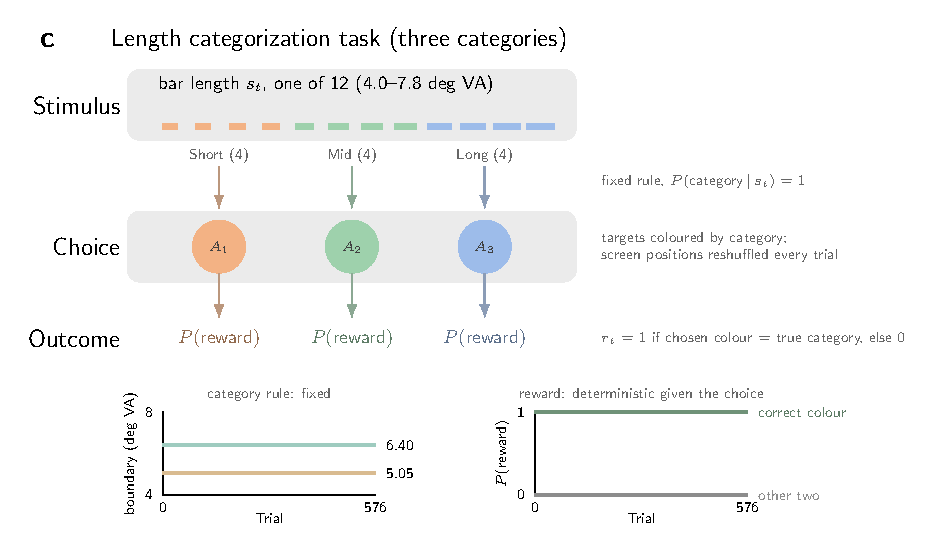
\includegraphics[width=0.9\textwidth]{panel_c.pdf}
  \caption{Task structure in the three-category framing. Twelve bar lengths, four per
  category, map deterministically onto Short, Mid and Long. The category boundaries
  (5.05 and 6.40 deg VA) are the nominal midpoints between adjacent lengths of different
  categories; they never change within or across sessions. Reward is deterministic
  given the choice. In the two-category framing (session mode \texttt{2cat}) the split
  is lengths 1--6 versus 7--12, with a single boundary at 5.85, and only the Short and
  Long targets are shown.}
  \label{fig:task}
\end{figure}

\begin{figure}[htbp]
  \centering
  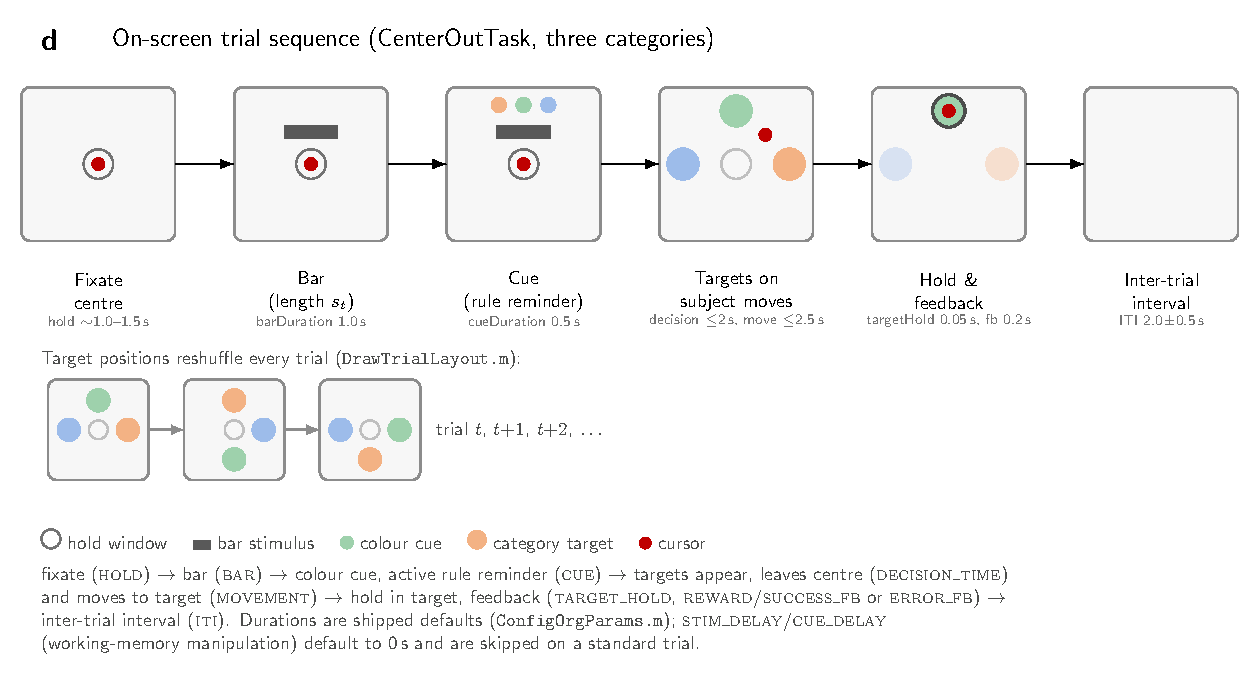
\includegraphics[width=\textwidth]{panel_d.pdf}
  \caption{On-screen sequence of one trial, following the epoch order in
  \texttt{TaskEpoch.m}: fixation at the centre, bar (1.0 s), colour cue (0.5 s, two or
  three dots that remind the subject of the active rule), target onset (go), movement,
  hold and feedback, inter-trial interval. The bar-to-go interval is essentially fixed
  (1.55 s, range 35 ms). Target positions reshuffle every trial, so repeating a category
  and repeating a direction are dissociable.}
  \label{fig:sequence}
\end{figure}

\subsection{What the task writes}

For every session the task writes \texttt{trial\_data\_<runTag>.csv} (one row per
trial), two trajectory exports at the cursor sampling rate (about 9 ms), a per-condition
summary and a text report. Only the trial table is used here. Its relevant columns are
listed in Table~\ref{tab:columns}.

\begin{table}[H]
  \centering\small
  \caption{Columns of \texttt{trial\_data\_*.csv} used by the model and their encoding.}
  \label{tab:columns}
  \begin{tabular}{lll}
    \toprule
    Model variable & Column & Encoding \\
    \midrule
    $s_t$        & \texttt{BarSizeVA\_deg}  & scalar, normalised to $[-1,1]$ over 4.0--7.8 \\
    $a_t$        & \texttt{ChosenTarget} (1 Short, 2 Mid, 3 Long, 0 none) & ordinal label $0/1/2$; none $\rightarrow$ masked \\
    $r_t$        & \texttt{IsCorrect}       & binary \\
    $\cue_t$     & \texttt{NumCategories} (2 or 3; absent in old schema $\rightarrow$ 3) & one-hot, 2 channels \\
    order        & \texttt{Block}, \texttt{TrialNumInBlock} & defines the sequence within a session \\
    retry        & \texttt{Attempt}         & only \texttt{Attempt} $=1$ is kept \\
    \bottomrule
  \end{tabular}
\end{table}

The history inputs are the same variables shifted by one trial: $a_{t-1}$, $s_{t-1}$,
$r_{t-1}$. The first trial of a session receives a ``no history'' vector (zeros plus an
indicator channel), never the last trial of the previous session.

\subsection{What the data show}

Thirteen sessions (20 August to 5 September 2026, subject ROM) hold 3\,866 trials, of
which 3\,818 have a response. Overall accuracy is 0.765 and is stable across sessions
(0.73--0.81). Errors are almost all wrong-target choices (860) rather than early exits
(48). Retries are rare (51).

\paragraph{Psychometric function.} Table~\ref{tab:psycho} pools the three-category
sessions. The subject's Short/Mid boundary sits below the nominal 5.05: at 4.70 it
already answers Mid half of the time. The Mid/Long boundary falls near the nominal 6.40.
A network fitted to behaviour must reproduce this asymmetry; a network trained on the
correct labels will not.

\begin{table}[H]
  \centering\small
  \caption{Probability of each response as a function of bar length, three-category
  sessions pooled ($n \approx 310$ per length).}
  \label{tab:psycho}
  \begin{tabular}{cccc}
    \toprule
    Length (deg VA) & $P(\Short)$ & $P(\Mid)$ & $P(\Long)$ \\
    \midrule
    4.00 & 0.98 & 0.01 & 0.01 \\
    4.10 & 0.96 & 0.02 & 0.02 \\
    4.70 & 0.42 & 0.52 & 0.07 \\
    5.00 & 0.23 & 0.66 & 0.11 \\
    5.10 & 0.15 & 0.75 & 0.10 \\
    5.70 & 0.04 & 0.79 & 0.17 \\
    6.00 & 0.03 & 0.78 & 0.19 \\
    6.10 & 0.02 & 0.68 & 0.30 \\
    6.70 & 0.02 & 0.19 & 0.79 \\
    7.00 & 0.00 & 0.09 & 0.90 \\
    7.60 & 0.01 & 0.02 & 0.97 \\
    7.80 & 0.02 & 0.03 & 0.96 \\
    \bottomrule
  \end{tabular}
\end{table}

\paragraph{Sequential effects are weak.} Accuracy is 0.788 after a correct trial and
0.692 after an error ($n = 2\,953$ and $913$). The probability of repeating the
previous category is 0.322 after a correct trial and 0.293 after an error, against a
chance level of $1/3$. The past therefore contributes little beyond a post-error effect.
This bounds what the network can find and motivates the small $d$ below.

\paragraph{The \texttt{alternate} regime is the base regime.} From 5 September onward
sessions run in session mode \texttt{alternate}: full 48-trial blocks of two and three
categories follow each other (the first such session ran 2, 2, 3, 3, 2, 2, 3). Accuracy
was 0.795 in the two-category blocks and 0.744 in the three-category blocks of that
session. This is the regime the network is designed for: identical stimuli, a rule that
changes within the day, signalled only by the cue, and a block switch every one to three
blocks. The design below assumes a corpus of \texttt{alternate} sessions of the same
size as the three-category corpus already recorded (12 to 15 sessions, 50 to 70 block
switches; the budget is derived in Section~\ref{sec:type}). The three-category-only sessions of August and early September are
kept as auxiliary training data (Section~\ref{sec:split}).

\paragraph{Filters.} Table~\ref{tab:filters} lists what is removed and why. After
filtering there are about 3\,750 labelled trials in the 12 sessions recorded so far,
190 of them in two-category blocks; the \texttt{alternate} corpus grows with every new
session.

\begin{table}[H]
  \centering\small
  \caption{Exclusions.}
  \label{tab:filters}
  \begin{tabular}{lp{8.5cm}r}
    \toprule
    Filter & Reason & Trials \\
    \midrule
    \texttt{Attempt} $>1$ & retries re-show a stimulus the subject just failed and distort the psychometric function & 51 \\
    \texttt{ChosenTarget} $=0$ & no choice to predict; the trial stays in the sequence as input to the next one but leaves the loss & 48 \\
    Session \texttt{28-Aug} & 21 trials, accuracy 0.33 & 21 \\
    \bottomrule
  \end{tabular}
\end{table}

%======================================================================
\section{Problem formulation}
%======================================================================

Each session is one sequence. At step $t$ the network receives $\vect{x}_t$, updates
its state $\vect{h}_t$ and outputs $\hat{\vect{y}}_t = P(a_t \mid \vect{x}_{1:t})$. This
is a many-to-many problem with $T_x = T_y$: one output per input step, with $T$ equal to
the number of trials in the session (240--465). It is neither many-to-one nor an
encoder--decoder (Figure~\ref{fig:m2m}).

The objective is the likelihood of the observed choices,
\begin{equation}
  \mathcal{L}(\theta) \;=\; -\frac{1}{N_{\mathrm{lab}}}
  \sum_{\text{sessions}} \sum_{t=1}^{T} m_t \,
  \log P_\theta\!\left(a_t = a_t^{\mathrm{obs}} \,\middle|\, \vect{x}_{1:t}\right),
  \qquad N_{\mathrm{lab}} = \sum m_t ,
  \label{eq:loss}
\end{equation}
where $m_t = 1$ if the trial has a response and \texttt{Attempt} $= 1$, and $m_t = 0$
otherwise. The network is not trained to solve the task; it is trained to predict what
the subject did, errors included.

\begin{figure}[htbp]
  \centering
  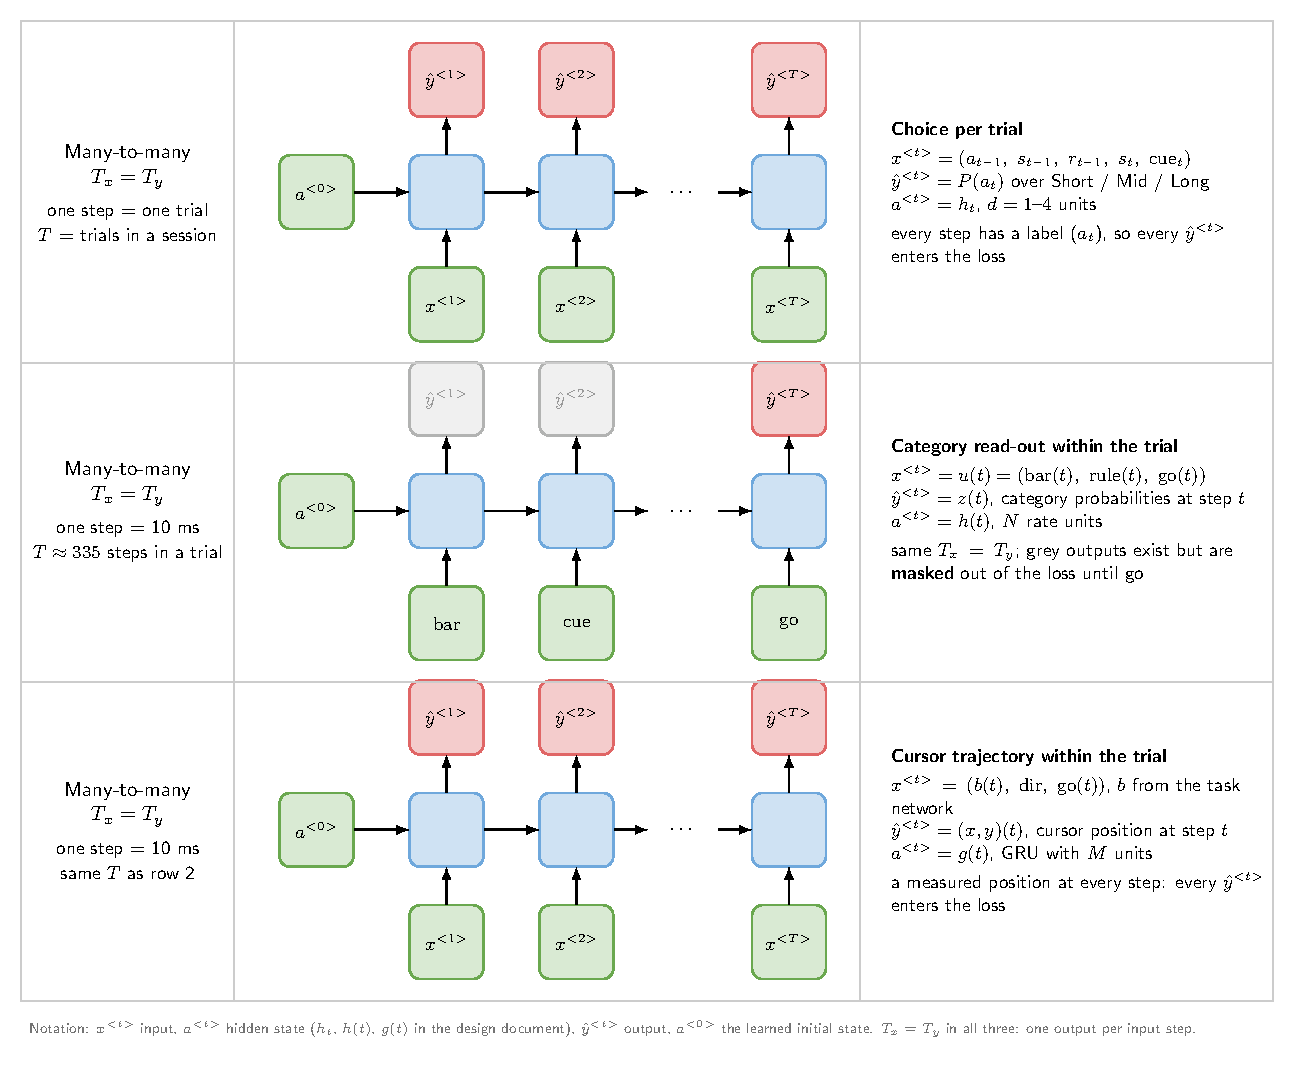
\includegraphics[width=0.8\textwidth]{panel_i.pdf}
  \caption{The three networks of the project in the standard many-to-many layout,
  $T_x = T_y$. Green boxes are inputs $x^{\langle t\rangle}$, blue boxes the hidden
  state $a^{\langle t\rangle}$ (our $\vect{h}_t$), red boxes the outputs
  $\hat y^{\langle t\rangle}$, and $a^{\langle 0\rangle}$ the learned initial state.
  Top row: this document's network, one step per trial. Middle and bottom rows: the
  within-trial task and motor networks of the companion document, one step per 10 ms;
  grey outputs exist but are masked out of the loss until the go signal.}
  \label{fig:m2m}
\end{figure}

%======================================================================
\section{Type of network, size, and data budget}
\label{sec:type}
%======================================================================

This section answers, in plain terms, what kind of recurrent network is used and why,
what its size parameter $d$ means, which activation functions it contains, and how many
sessions are needed. The formal equations follow in Section~\ref{sec:arch}.

\subsection{Which kind of recurrent network}

A recurrent network is any model in which a state vector is updated at every step from
its previous value and the current input. Three standard cells differ in how the update
is written.

\begin{itemize}[leftmargin=*]
\item \textbf{Vanilla (Elman) RNN.} One equation,
      $\vect{h}_t = \tanh(\vect{W}\vect{x}_t + \vect{U}\vect{h}_{t-1} + \vect{b})$.
      Keeping a value and replacing it go through the same weights, so a unit cannot
      do both well, and gradients through hundreds of steps vanish or explode.
\item \textbf{GRU (gated recurrent unit).} The same state, plus two gates that decide,
      per unit and per step, how much of the old value to keep and how much to
      overwrite (Eqs.~\eqref{eq:gru-r}--\eqref{eq:gru-h}). One state vector, three
      weight sets.
\item \textbf{LSTM.} Two state vectors (cell and hidden) and three gates. More
      parameters, and the ``number of state variables'' is ambiguous because each unit
      carries two numbers.
\end{itemize}

\textbf{The network is a GRU, not a vanilla RNN.} Three reasons. It is the cell used by
Ji-An et al., so the comparison with their results is direct. With $d = 1$ or $2$ the
gates are what let a single unit hold a criterion across trials and still reset it after
an error or a cue; a vanilla unit has to choose one behaviour. And it has one state
vector, so $d$ is unambiguous. The LSTM is not used because it doubles the state for no
gain at this size. A vanilla RNN with the same $d$ is fitted as a control
(Section~\ref{sec:models}): with short memory the gates may not be needed, and if the
two cells tie, the vanilla one is preferred because its dynamics are easier to read.

\subsection{What $d$ is}

$d$ is the number of hidden units, which for a GRU equals the dimension of the state
vector $\vect{h}_t \in \mathbb{R}^d$, which in turn equals the number of dynamical
variables: the number of quantities the model carries from one trial to the next. In the
framing of Ji-An et al.\ this number, not the parameter count, is the measure of model
complexity, because it is what a cognitive model also has: the criterion-shift model M2
has $d = 2$ (two boundaries), the Bayesian observer $d = 4$ (mean and width of each
boundary), a model-free learner $d = 36$ (one value per length and category). Two models
with the same $d$ can be compared on equal terms even if one has twenty parameters and
the other eighty, because they remember the same amount and differ only in the form of
the update.

With $d = 1$ the entire memory of the animal, as the model sees it, is a single number
that moves up and down across trials. That is deliberately restrictive: it is the case in
which the whole dynamics can be drawn on a page. The prediction for this task is that
$d = 1$ or $2$ is enough, because the rule is fixed and sequential effects are weak.
$d = 3$ and $4$ are fitted to confirm that they do not improve held-out likelihood.

\subsection{What a hidden unit is here}

A hidden unit is one coordinate of $\vect{h}_t$: a scalar that is read from the previous
trial, updated with the current inputs, and passed on. It is not a neuron and it is not
a feature detector. In this network a unit is expected to behave as a slowly varying
bias, for instance the current displacement of a criterion from its resting value.
Units have no assigned meaning before training; their meaning is established afterwards
by reading how they move the criteria (Section~\ref{sec:interp}). That is the difference
between the $h_t$ of the network and the $V_t$ or $c_t$ of a cognitive model, which are
named before any data are seen.

\subsection{Activation functions, and why those}

There are three places where a nonlinearity sits, and only one of them is a choice.

\begin{itemize}[leftmargin=*]
\item \textbf{Gates: logistic $\sigma$.} A gate is a proportion, how much to keep and
      how much to replace, so it must lie in $(0,1)$. The logistic function is the
      standard map onto that interval. Fixed by the GRU definition.
\item \textbf{Candidate state: $\tanh$.} The state must be bounded, otherwise it can
      grow without limit over the 300 steps of a session, and it must be symmetric
      around zero so that a criterion can move in either direction. $\tanh$ gives both;
      a ReLU would give neither. Fixed by the GRU definition.
\item \textbf{Read-out: logistic or cumulative Gaussian.} Each criterion turns a
      distance on the length axis into a probability, so the read-out is a sigmoid
      curve; it is the psychometric function of the model. Logistic and cumulative
      Gaussian are both used in psychophysics and differ only by a scale factor of about
      1.7 in the slope. The logistic is the default; the Gaussian is used when an exact
      match with the notebook's psychometric fits is wanted. This is the one choice.
\end{itemize}

No softmax is used: the ordinal read-out already yields three probabilities that sum to
one, and a softmax would discard the ordering of the categories.

\subsection{Size of the network and of the data}

The network has $d$ units, $k = 9$ (or 10) input channels and between 42 and 189
learned parameters (Table~\ref{tab:params}). Each session is one sequence of 240 to 465
steps, and gradients are propagated through the whole session. This is small: a fit
takes seconds, and the whole grid of models, folds and seeds fits in an afternoon.

The data requirement is set by three needs, and the largest of them decides.

\begin{enumerate}[leftmargin=*]
\item \textbf{Trials per parameter.} A rule of thumb for a well-conditioned
      maximum-likelihood fit is at least 20 labelled trials per parameter. With
      $d = 2$ and 85 parameters that is 1\,700 trials, about six sessions. The
      three-category sessions already recorded cover this for the choice model alone.
\item \textbf{Outer folds.} The paired comparison between models uses one difference
      per test session. Ten differences are the minimum for a bootstrap interval that
      means anything; twelve to fifteen are comfortable.
\item \textbf{Block switches.} The rule questions are answered on the trials after
      each switch. With segment lengths drawn from one to three blocks and about 320
      trials per session, a session holds
      $\approx 320 / \bar{L} - 1$ switches, where $\bar{L}$ is the mean segment length
      in trials. With segments mostly of one block ($\bar{L} \approx 65$) that is four
      to five switches per session; with segments averaging two blocks it is two to
      three. To estimate the post-switch curve on five trials, in both directions
      (2$\to$3 and 3$\to$2), with a resolution of about one trial in the time
      constant, at least 50 to 60 switches are needed.
\end{enumerate}

Need 3 dominates. \textbf{The target is 12 to 15 \texttt{alternate} sessions, with
segment lengths drawn from $\{1, 2, 3\}$ blocks with weights about $0.6/0.3/0.1$},
which yields four to five switches per session and 50 to 70 switches in total, and at the
same time satisfies needs 1 and 2. Ten sessions is the floor below which the latent-rule
version (Section~\ref{sec:rule}) cannot be fitted with confidence; the cue-driven
version and the choice-only questions are already answerable with the sessions recorded.
The three-category-only sessions add to need 1 but not to needs 2 and 3.

%======================================================================
\section{Architecture}
\label{sec:arch}
%======================================================================

\subsection{Overview}

Figure~\ref{fig:panel_a} places the network next to a cognitive model in the framing of
Ji-An et al.: both are dynamical systems with $d$ state variables, the same inputs and
the same output. They differ only in who writes the update rule. In the cognitive model
the variables have a meaning fixed in advance (here, decision criteria $c_t$) and the
update rule is written by the modeller; in the network the variables $\vect{h}_t$ have
no assigned meaning and the update rule is learned.

\begin{figure}[htbp]
  \centering
  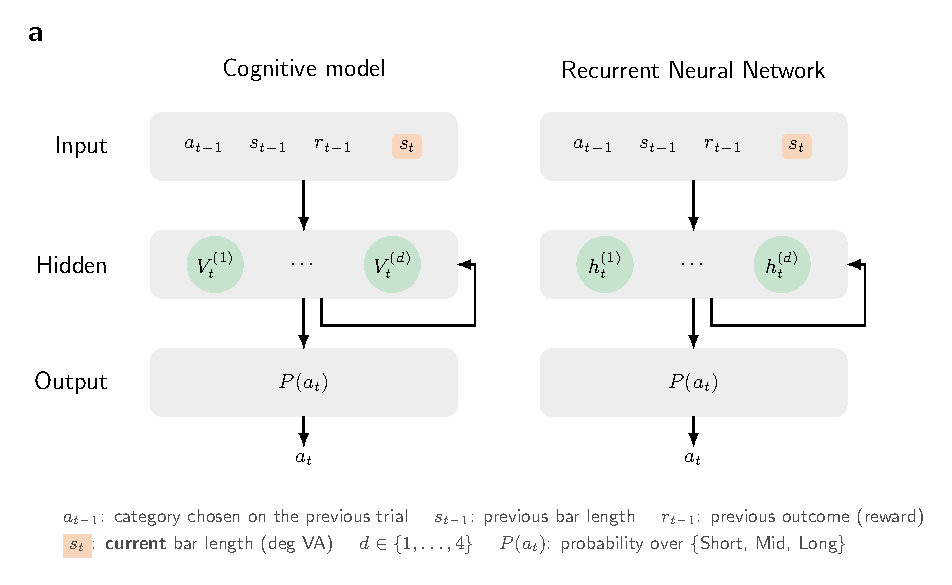
\includegraphics[width=0.95\textwidth]{panel_a.pdf}
  \caption{Trial-level model. Left: a cognitive model whose $d$ state variables
  $V_t^{(i)}$ carry a meaning assigned by the modeller (for this task, decision
  criteria). Right: the recurrent network, whose $d$ hidden units $h_t^{(i)}$ are
  interpreted after training. Both receive the previous choice $a_{t-1}$, the previous
  bar length $s_{t-1}$, the previous outcome $r_{t-1}$ and, highlighted, the current
  bar length $s_t$, the input the reward-learning tasks of Ji-An et al.\ do not have.
  Both output a probability over Short, Mid and Long.}
  \label{fig:panel_a}
\end{figure}

\subsection{Inputs}

The input vector has $k = 9$ channels (Table~\ref{tab:inputs}).

\begin{table}[H]
  \centering\small
  \caption{Input channels $\vect{x}_t$.}
  \label{tab:inputs}
  \begin{tabular}{llp{8cm}}
    \toprule
    Channel & Dim. & Content \\
    \midrule
    $s_t$        & 1 & current bar length, normalised \\
    $s_{t-1}$    & 1 & previous bar length, normalised \\
    $a_{t-1}$    & 3 & one-hot of the previously chosen category \\
    $r_{t-1}$    & 1 & 1 if the previous choice was rewarded \\
    $\cue_t$     & 2 & one-hot: two categories / three categories \\
    first        & 1 & 1 on the first trial of a session \\
    \midrule
    total $k$    & 9 & \\
    \midrule
    $\log \mathrm{DT}_{t-1}$ (optional) & 1 & previous decision time, standardised; Section~\ref{sec:dt} \\
    \bottomrule
  \end{tabular}
\end{table}

\paragraph{Design decision: $s_t$ enters twice.} The current length is fed both to the
recurrent cell and directly to the read-out (Section~\ref{sec:readout}). With $d = 1$
or $2$, if $s_t$ entered only through the cell, the unit would be spent representing
the stimulus and no memory would remain. The direct connection leaves the cell free to
represent only what changes from trial to trial.

\paragraph{What is left out.} \texttt{PrevTrialDirection} is logged but not used: without
an export of the target layout it cannot be related to the chosen category. It becomes
usable once the layout is exported (Section~\ref{sec:data-req}).

\subsection{State: a gated recurrent unit}
\label{sec:gru}

The state is updated by a GRU cell (Figure~\ref{fig:gru}):
\begin{align}
  \vect{r}_t &= \sigma\!\left(\vect{W}_r \vect{x}_t + \vect{U}_r \vect{h}_{t-1} + \vect{b}_r\right)
    && \text{reset gate} \label{eq:gru-r}\\
  \vect{z}_t &= \sigma\!\left(\vect{W}_z \vect{x}_t + \vect{U}_z \vect{h}_{t-1} + \vect{b}_z\right)
    && \text{update gate} \label{eq:gru-z}\\
  \tilde{\vect{h}}_t &= \tanh\!\left(\vect{W}_h \vect{x}_t + \vect{U}_h\,(\vect{r}_t \odot \vect{h}_{t-1}) + \vect{b}_h\right)
    && \text{candidate} \label{eq:gru-c}\\
  \vect{h}_t &= (1 - \vect{z}_t) \odot \vect{h}_{t-1} + \vect{z}_t \odot \tilde{\vect{h}}_t
    && \text{new state} \label{eq:gru-h}
\end{align}
with $\sigma$ the logistic function, $\odot$ the element-wise product, and
$\vect{h}_t \in \mathbb{R}^d$.

\begin{figure}[htbp]
  \centering
  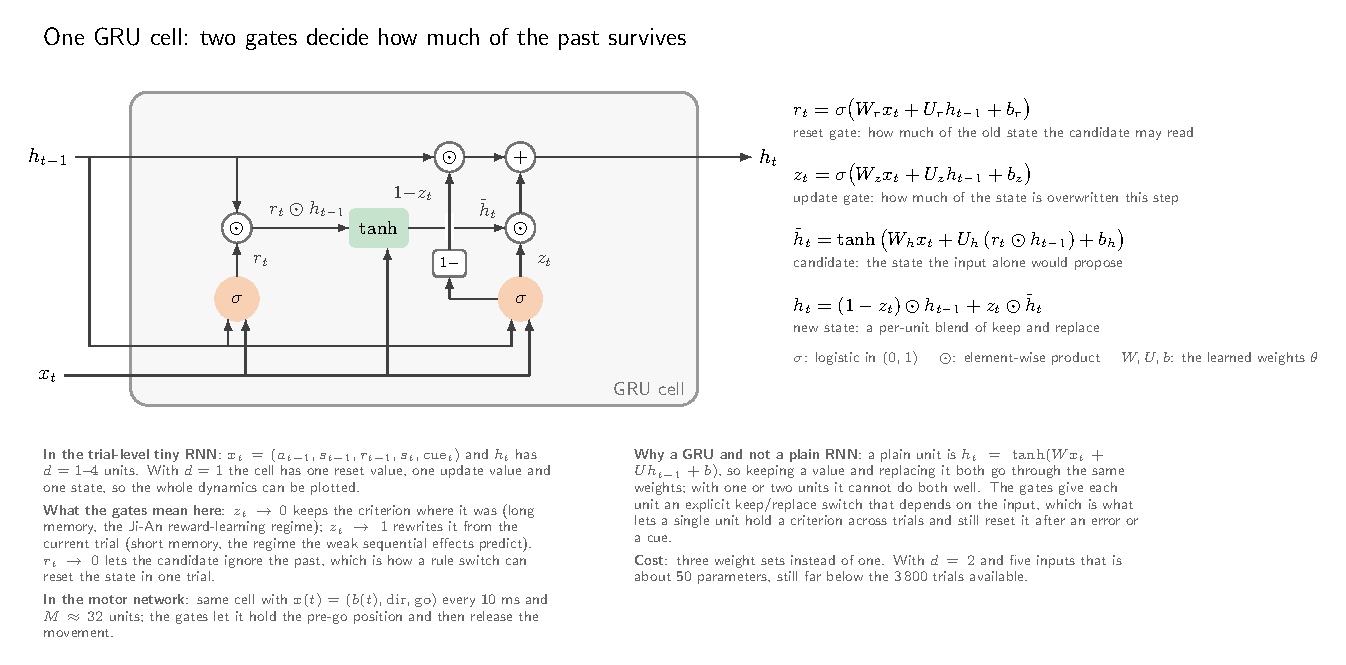
\includegraphics[width=\textwidth]{panel_h.pdf}
  \caption{One GRU cell. The reset gate $r_t$ decides how much of the old state the
  candidate may read; the update gate $z_t$ decides how much of the state is
  overwritten; the new state is a per-unit blend of keep and replace. In this task,
  $z_t \to 0$ keeps a criterion where it was (long memory, the reward-learning regime
  of Ji-An et al.), $z_t \to 1$ rewrites it from the current trial (short memory, the
  regime the weak sequential effects predict), and $r_t \to 0$ lets the candidate ignore
  the past, which is how a rule switch can reset the state in a single trial.}
  \label{fig:gru}
\end{figure}

\begin{table}[H]
  \centering\small
  \caption{Decisions about the recurrent cell.}
  \begin{tabular}{lp{5cm}p{7.5cm}}
    \toprule
    Element & Decision & Justification \\
    \midrule
    Cell type & GRU & Same as Ji-An et al., so the comparison is clean; with small $d$ the gates let a single unit both hold and reset \\
    Comparison & plain RNN $\vect{h}_t = \tanh(\vect{W}\vect{x}_t + \vect{U}\vect{h}_{t-1} + \vect{b})$, same $d$ & With short memory the advantage of gating may vanish; if the two tie, the plain cell is preferred for interpretability \\
    $d$ & 1, 2, 3, 4, one at a time & The main complexity axis. Prediction: 1 or 2 suffice \\
    $\vect{h}_0$ & learned vector shared across sessions & The start of a session is the same ``no history'' state everywhere \\
    Activations & $\sigma$ in the gates, $\tanh$ in the candidate & Fixed by the GRU definition: proportions in $(0,1)$, a bounded and symmetric state \\
    \bottomrule
  \end{tabular}
\end{table}

\subsection{Read-out: ordinal with two criteria}
\label{sec:readout}

The categories are ordered along the length axis, so the output is parameterised as a
perceived length and two criteria rather than three free logits:
\begin{align}
  \hat{x}_t &= g(s_t, \vect{h}_t) = s_t + \vect{w}_g\T \vect{h}_t + b_g
    && \text{perceived length} \label{eq:ro-x}\\
  c_1(\vect{h}_t) &= c_1^{0} + \vect{w}_1\T \vect{h}_t
    && \text{first criterion} \label{eq:ro-c1}\\
  c_2(\vect{h}_t) &= c_1(\vect{h}_t) + \operatorname{softplus}\!\left(\delta^{0} + \vect{w}_2\T \vect{h}_t\right)
    && \text{second criterion, } c_2 \ge c_1 \label{eq:ro-c2}\\
  P(a_t \ge k) &= (1-\lambda)\,F\!\left(\beta\,(\hat{x}_t - c_k)\right) + \tfrac{\lambda}{2},
    \qquad k = 1, 2 \label{eq:ro-p}
\end{align}
and the category probabilities follow from the cumulative ones:
\begin{equation}
  P(a_t = \Short) = 1 - P(a_t \ge 1), \qquad
  P(a_t = \Mid)   = P(a_t \ge 1) - P(a_t \ge 2), \qquad
  P(a_t = \Long)  = P(a_t \ge 2).
  \label{eq:ro-cat}
\end{equation}

\begin{table}[H]
  \centering\small
  \caption{Decisions about the read-out.}
  \begin{tabular}{lp{5cm}p{7.5cm}}
    \toprule
    Element & Decision & Justification \\
    \midrule
    Form & cumulative ordinal & Same structure as the criterion cognitive model and as the notebook's psychometric fit, which uses the ordinal splits $P(\text{chosen} \ge k)$ \\
    $F$ & logistic by default; cumulative Gaussian as an option & Logit and probit differ by a factor of about 1.7 in slope; the Gaussian matches the notebook exactly \\
    $\beta$ & learned slope, shared by both criteria & Perceptual sensitivity \\
    $\lambda$ & learned lapse, bounded in $[0, 0.1]$ & Stimulus-independent errors; without it the slope absorbs the lapses \\
    Order $c_2 \ge c_1$ & softplus parameterisation, Eq.~\eqref{eq:ro-c2} & Guarantees a non-negative probability for Mid \\
    Two-category blocks & same read-out, nothing masked & $P(\Mid) = P(a \ge 1) - P(a \ge 2)$ vanishes when $c_1 \to c_2$: the network learns to collapse the criteria onto 5.85 \\
    \bottomrule
  \end{tabular}
\end{table}

\paragraph{Separation of biases.} Whatever enters through $g$ shifts \emph{perception}
and affects both rules equally (serial dependence on $s_{t-1}$). Whatever enters
through $c_k$ shifts the \emph{decision} (post-error shift, rule). This separation is
written into the architecture and is read directly from the weights $\vect{w}_g$
versus $\vect{w}_1, \vect{w}_2$.

\subsection{Activation functions}

No softmax is used: the ordinal read-out already produces a distribution that sums to
one.

\begin{table}[H]
  \centering\small
  \caption{Where each activation function sits and whether it is a choice.}
  \begin{tabular}{llll}
    \toprule
    Place & Function & Range & Chosen or fixed \\
    \midrule
    Gates $\vect{r}_t$, $\vect{z}_t$ & logistic & $(0,1)$ & fixed (GRU) \\
    Candidate $\tilde{\vect{h}}_t$ & $\tanh$ & $(-1,1)$ & fixed (GRU) \\
    Perceived length $\hat x_t$ & linear & $\mathbb{R}$ & fixed (a position on the axis) \\
    Criteria $c_k$ & linear & $\mathbb{R}$ & fixed \\
    Cumulative probability & logistic or cumulative Gaussian & $(0,1)$ & chosen \\
    \bottomrule
  \end{tabular}
\end{table}

\subsection{Learned parameters}

With $k = 9$ input channels the parameter counts are those of
Table~\ref{tab:params}. With about 3\,750 labelled trials there are between 20 and 90
trials per parameter, enough for $d \le 2$. The $d = 4$ configuration needs stronger
regularisation and is included to confirm that it does not improve.

\begin{table}[H]
  \centering\small
  \caption{Number of learned parameters.}
  \label{tab:params}
  \begin{tabular}{llrrr}
    \toprule
    Block & Formula & $d=1$ & $d=2$ & $d=4$ \\
    \midrule
    GRU & $3\,(dk + d^2 + d)$ & 33 & 72 & 168 \\
    $\vect{h}_0$ & $d$ & 1 & 2 & 4 \\
    Read-out $g$ & $d + 1$ & 2 & 3 & 5 \\
    Criteria & $2\,(d + 1)$ & 4 & 6 & 10 \\
    $\beta$, $\lambda$ & 2 & 2 & 2 & 2 \\
    \midrule
    Total & & 42 & 85 & 189 \\
    \bottomrule
  \end{tabular}
\end{table}

%======================================================================
\section{Two ways of knowing the rule}
\label{sec:rule}
%======================================================================

The subject sees two or three dots in the cue and two or three targets on screen.
Giving that information to the network is not cheating: it models a subject who reads
the cue. Withholding it forces the network to infer the rule from feedback, which is
what the networks of Ji-An et al.\ do in reversal tasks. Both versions are fitted
(Table~\ref{tab:rule}, Figure~\ref{fig:rule}).

\begin{table}[H]
  \centering\small
  \caption{The two rule versions.}
  \label{tab:rule}
  \begin{tabular}{llp{4.5cm}p{5.5cm}}
    \toprule
    Version & $\cue_t$ & Models & Distinctive prediction \\
    \midrule
    Cue-driven (main) & input channel & a subject who reads the cue & criteria move on the trial of the block switch \\
    Feedback-inferred & channel off & a subject who infers the rule from errors & criteria drift over several trials until they collapse onto 5.85 \\
    \bottomrule
  \end{tabular}
\end{table}

The cue-driven version is the ceiling: the latent version cannot beat it, and the
question is how close it gets and with what delay. A third reading comes for free: if,
even with the cue given, the learned dynamics show gradual carry-over, the subject does
not fully use the cue.

\begin{figure}[htbp]
  \centering
  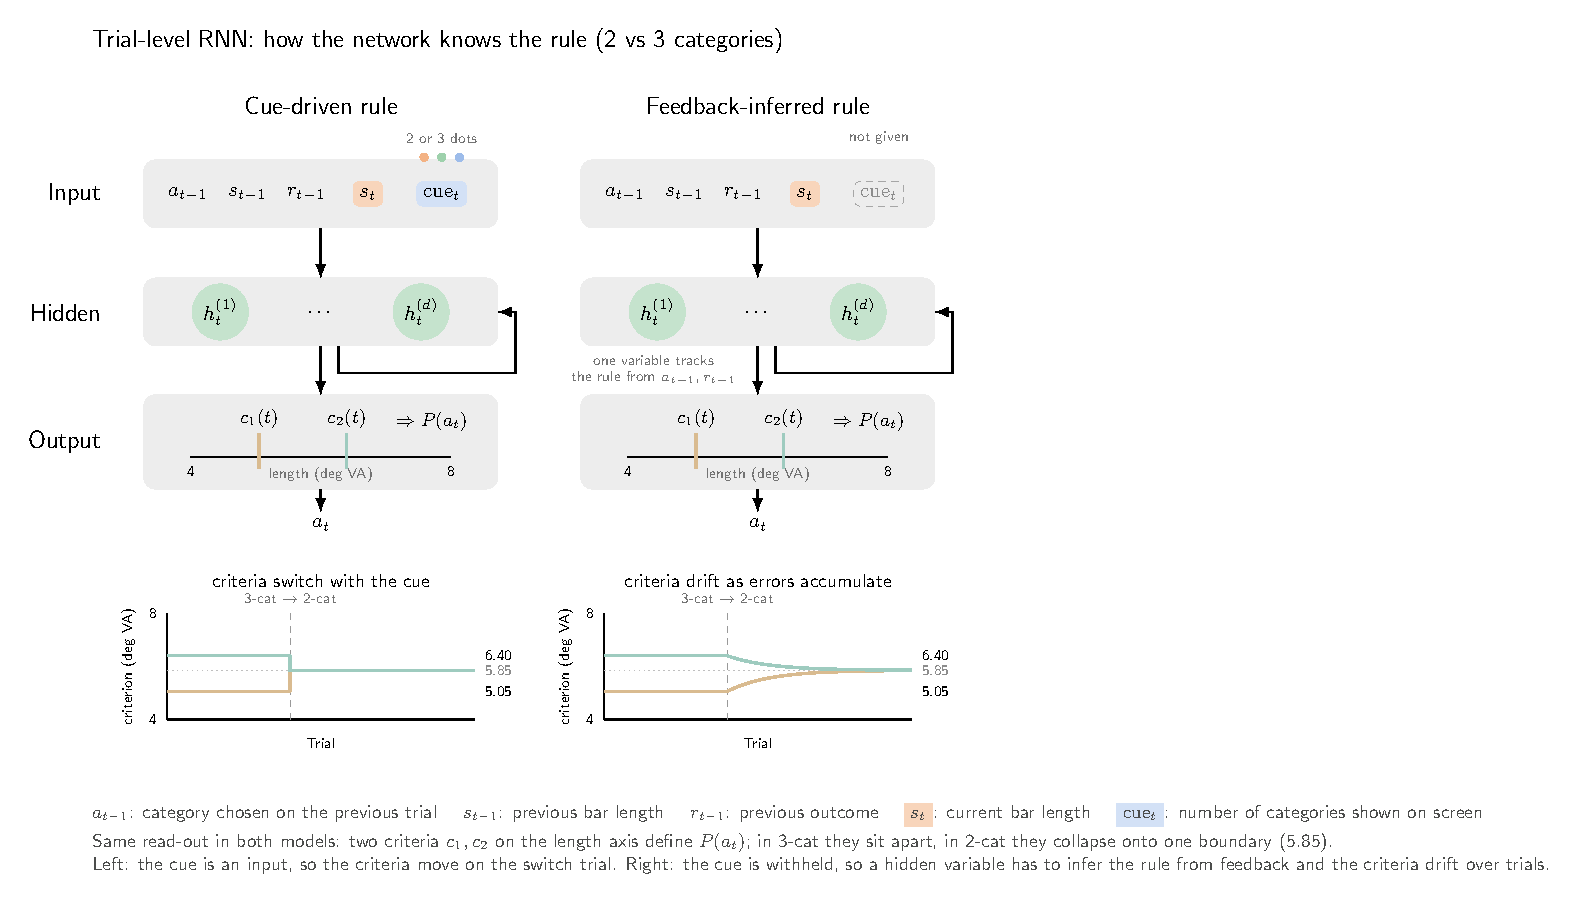
\includegraphics[width=0.95\textwidth]{panel_e.pdf}
  \caption{Cue-driven versus feedback-inferred rule. Both networks share the ordinal
  read-out with two criteria $c_1, c_2$ on the length axis. Left: the cue is an input,
  so the criteria can jump from the three-category positions (5.05, 6.40) to the
  two-category position (5.85) on the switch trial. Right: the cue is withheld, so a
  hidden variable must infer the rule from $a_{t-1}, r_{t-1}$ and the criteria drift as
  errors accumulate. The lower plots are the predicted criterion trajectories around a
  block switch; once fitted, the same plot is produced from the data.}
  \label{fig:rule}
\end{figure}

%======================================================================
\section{Decision time as a second observable}
\label{sec:dt}
%======================================================================

The trial table logs, for every trial with a response, the time from target onset to
leaving the centre (\texttt{DecisionTime\_s}, median 351 ms, 5th--95th percentile
292--492 ms) and the time from leaving the centre to reaching the target
(\texttt{ExecutionTime\_s}, median 183 ms). The first is the time of the decision; the
second is motor and is left to the motor network of the companion document. The decision
time can enter the model in two ways, which answer different questions.

\subsection{The previous decision time as an input}

$\mathrm{DT}_{t-1}$ is observed before trial $t$, so it can be an input channel without
any leakage. It carries something $a_{t-1}$ and $r_{t-1}$ do not: how sure the subject
was. A slow correct choice and a fast correct choice are different histories, and the
criterion shift may depend on that. The channel is $\log \mathrm{DT}_{t-1}$,
standardised within the training set, set to zero on trials without a response; the
input dimension becomes $k = 10$. It is tested with the same ablation as the other
channels.

What cannot be done is to use $\mathrm{DT}_t$, the current trial's time, as an input for
predicting $a_t$: it is part of the same response that is being predicted.

\subsection{The current decision time as a second output}

The more informative use is to predict choice and decision time jointly from the same
state. The decision time is modelled as log-normal with a mean that depends on the
distance from the perceived length to the nearest criterion:
\begin{align}
  D_t &= -\min_{k \in \{1,2\}} \left|\, \hat{x}_t - c_k(\vect{h}_t) \,\right|
    && \text{proximity to the nearest criterion} \label{eq:dt-D}\\
  \mu_t &= \mu_0 + \kappa\, D_t + \vect{w}_{\mathrm{DT}}\T \vect{h}_t
    && \text{predicted log decision time} \label{eq:dt-mu}\\
  \log \mathrm{DT}_t &\sim \mathcal{N}\!\left(\mu_t, \sigma_{\mathrm{DT}}^2\right)
    && \label{eq:dt-lik}
\end{align}
with learned $\mu_0$, $\kappa$, $\vect{w}_{\mathrm{DT}}$ and $\sigma_{\mathrm{DT}}$.
The loss of Eq.~\eqref{eq:loss} gains a second term,
\begin{equation}
  \mathcal{L}(\theta) \;=\; \mathcal{L}_{\mathrm{choice}}(\theta)
  \;+\; \lambda_{\mathrm{RT}}\, \mathcal{L}_{\mathrm{DT}}(\theta), \qquad
  \mathcal{L}_{\mathrm{DT}} = \frac{1}{N_{\mathrm{lab}}} \sum m_t
  \left[ \frac{(\log \mathrm{DT}_t - \mu_t)^2}{2\sigma_{\mathrm{DT}}^2}
         + \log \sigma_{\mathrm{DT}} \right],
  \label{eq:loss-joint}
\end{equation}
with $\lambda_{\mathrm{RT}}$ chosen on the validation session so that neither term
dominates (start at $\lambda_{\mathrm{RT}} = 1$ with both terms in nats per trial). The
same mask $m_t$ applies: trials without a response have no decision time.

Three reasons to do this.

\begin{enumerate}[leftmargin=*]
\item \textbf{A second observation per trial.} With one categorical label per trial,
      the choice constrains the hidden state weakly. The decision time is continuous and
      constrains it far more. The joint fit is expected to identify $d$ and the
      criterion dynamics with less data.
\item \textbf{A direct test of the criterion interpretation.} If $c_1$ and $c_2$ are
      the subject's boundaries, decision times must peak where $\hat{x}_t$ falls near
      them. That is the chronometric function of the notebook (Section 1.6), computed
      with the model's boundaries instead of the nominal ones. A model that predicts
      the choice well and the time badly has criteria that are not the subject's.
      Equation~\eqref{eq:dt-D} makes the test explicit: $\kappa$ should be positive.
\item \textbf{A link to the task network.} The within-trial task network produces a
      decision time as the moment its read-out crosses a threshold. The trial-level
      $\mu_t$ and the within-trial crossing time must agree trial by trial; if they do
      not, one of the two networks carries a bias the other does not.
\end{enumerate}

To keep the comparison with the cognitive models fair, $\mathcal{L}_{\mathrm{choice}}$
is always reported on its own, and the criterion model M2 receives the same decision-time
read-out, Eqs.~\eqref{eq:dt-D}--\eqref{eq:dt-lik}, which it can because it also has
criteria. Models without criteria (M3) get $\mu_t = \mu_0 + \vect{w}\T \vect{Q}_t(s_t,\cdot)$.

\subsection{Elapsed time as an input}

The interval between trials is not constant: 2.0 s after a correct trial, 3.0 s after an
error, plus pauses. If the memory of the criterion decays with real time rather than with
trial count, a channel with $\Delta t$ since the previous trial lets the GRU learn a
time-dependent forgetting. The value comes from \texttt{Time\_ms} in the trajectory
export, not from the trial table. It is added last, and only if the ablation of
$r_{t-1}$ suggests decay.

\paragraph{Order of adoption.} First $\mathrm{DT}_{t-1}$ as an input, because it is one
more ablation and nothing else changes. Then the joint choice--time model, because that
is where the scientific gain is. Then $\Delta t$, if needed.

%======================================================================
\section{Training}
%======================================================================

\begin{table}[H]
  \centering\small
  \caption{Training protocol.}
  \begin{tabular}{lp{5.5cm}p{7cm}}
    \toprule
    Element & Value & Justification \\
    \midrule
    Loss & negative log-likelihood per trial, Eq.~\eqref{eq:loss} & It is what is compared across models \\
    Optimiser & Adam, learning rate $10^{-3}$, gradient clipping at 1.0 & Standard; sequences are long and clipping prevents blow-ups \\
    Batch & one whole session per sequence; batches of 4 sessions & The state must run through the session uncut, so that carry-over across blocks is observable \\
    Early stopping & on validation NLL, patience 50 epochs & Replaces a fixed epoch count; prevents memorisation \\
    Regularisation & L2 $10^{-4}$ on all weights; L1 $10^{-4}$ on $\vect{w}_g$, $\vect{w}_1$, $\vect{w}_2$ & Pushes state-to-read-out connections that do not help to zero, which simplifies interpretation \\
    Seeds & 10 per configuration; best on validation reported, with the spread & With $d=1$ the loss landscape has local optima \\
    Distillation (optional) & teacher GRU $d=16$ $\rightarrow$ student $d=1,2$ on the same sequences & Used by Ji-An et al.\ with scarce data; data are scarce here \\
    Split & nested cross-validation by session, Section~\ref{sec:split} & The unit of independence is the day, not the trial \\
    Report & mean test NLL per trial averaged over folds, bootstrap interval over sessions & \\
    \bottomrule
  \end{tabular}
\end{table}

Trials without a response and retries remain in the sequence as input to the following
trial; the mask $m_t = 0$ only removes them from the loss. Removing them from the
sequence would break the history the subject actually experienced.

\subsection{Data split: nested cross-validation by session}
\label{sec:split}

\paragraph{Why the unit is the session.} The state $\vect{h}_t$ runs through the whole
session, so consecutive trials are dependent by construction. A day also has effects of
its own that are not in the inputs: criterion drift, fatigue, joystick calibration. A
split by trial would let the model learn the state of the day from the training trials
and use it on the test trials of the same day, which inflates the likelihood and says
nothing about generalisation. A split by trial is defensible with tens of thousands of
trials per animal, as in the data of Ji-An et al.; it is not with about 300 trials per
day.

\paragraph{Corpus.} Two sets of sessions enter the fit. The \texttt{alternate}
sessions are the target corpus: every question of Section~\ref{sec:purpose} is answered on them. The
three-category-only sessions are auxiliary: they enter training with
$\cue_t = (0, 1)$ throughout, add about 3\,500 trials of psychometric structure, and are
never used as test for any question that involves the rule.

\paragraph{Outer loop: leave one \texttt{alternate} session out.} With $S$
\texttt{alternate} sessions there are $S$ folds. In each fold one \texttt{alternate}
session is the test set and is not touched during fitting. The remaining $S-1$
\texttt{alternate} sessions plus all auxiliary sessions form the fitting set. Test NLL
per trial, averaged over folds, is the number reported for every model. This measures
generalisation to a new day.

\paragraph{Inner loop: one validation session.} Inside the fitting set, one
\texttt{alternate} session is set aside as validation. It drives early stopping and the
choice of regularisation strength and seed. It is rotated over the $S-1$ candidates and
the resulting models are averaged in NLL, or, if compute is short, fixed to the session
closest in date to the test session. The number of state variables $d$ is \emph{not}
selected in the inner loop: $d$ is the quantity of interest, so every value is fitted
separately and its outer test NLL is reported.

\paragraph{Paired comparison.} All models of Section~\ref{sec:models} are evaluated on the same
folds. The difference in NLL between two models on each test session gives $S$ paired
values; the confidence interval is a bootstrap over those $S$ differences. Day-to-day
variation in absolute NLL cancels in the pairing.

\paragraph{Chronological check.} In addition to the random leave-one-out, a
forward-chaining pass: fit on all sessions before day $j$, test on day $j$, for every
$j$ from the third \texttt{alternate} session onward. If the chronological NLL is worse
than the leave-one-out NLL, the subject is still changing between days and the report
says so.

\paragraph{Secondary measure: blocks held out within a session.} For the dynamics
right after a block switch (Section~\ref{sec:interp}, items 1 and 2) the outer folds are complemented by
a within-session evaluation: in each \texttt{alternate} session, every second
two-category block and every second three-category block is masked out of the loss
while the network still reads it as input, and the NLL on the five trials after each
masked switch is reported separately. This is the masked trial-level split, and it is
legitimate here because the question is ``within this day, does the model predict the
trials that follow a switch?''. It is reported apart from the outer result, never
mixed with it.

\paragraph{The day-specific component.} The gap between the within-session NLL (blocks
held out) and the between-session NLL (day held out) is a direct measure of what is
specific to the day and not carried by the inputs. If it is small, the model transfers
across days. If it is large, there is a state of the day the network cannot infer from
the history, which motivates a per-session parameter or more sessions.

\paragraph{Cost.} With $S = 10$ outer folds, four values of $d$, ten seeds and eight
models the grid is about 3\,200 fits. Each fit takes seconds on networks of this size.

%======================================================================
\section{Comparison models}
\label{sec:models}
%======================================================================

All comparison models receive the same inputs, produce the same output and are fitted
with the same loss and the same split. They are compared by held-out NLL, at matched
$d$ where applicable. Figure~\ref{fig:four} shows how each one operationalises the same
problem; Table~\ref{tab:models} lists them.

\begin{figure}[htbp]
  \centering
  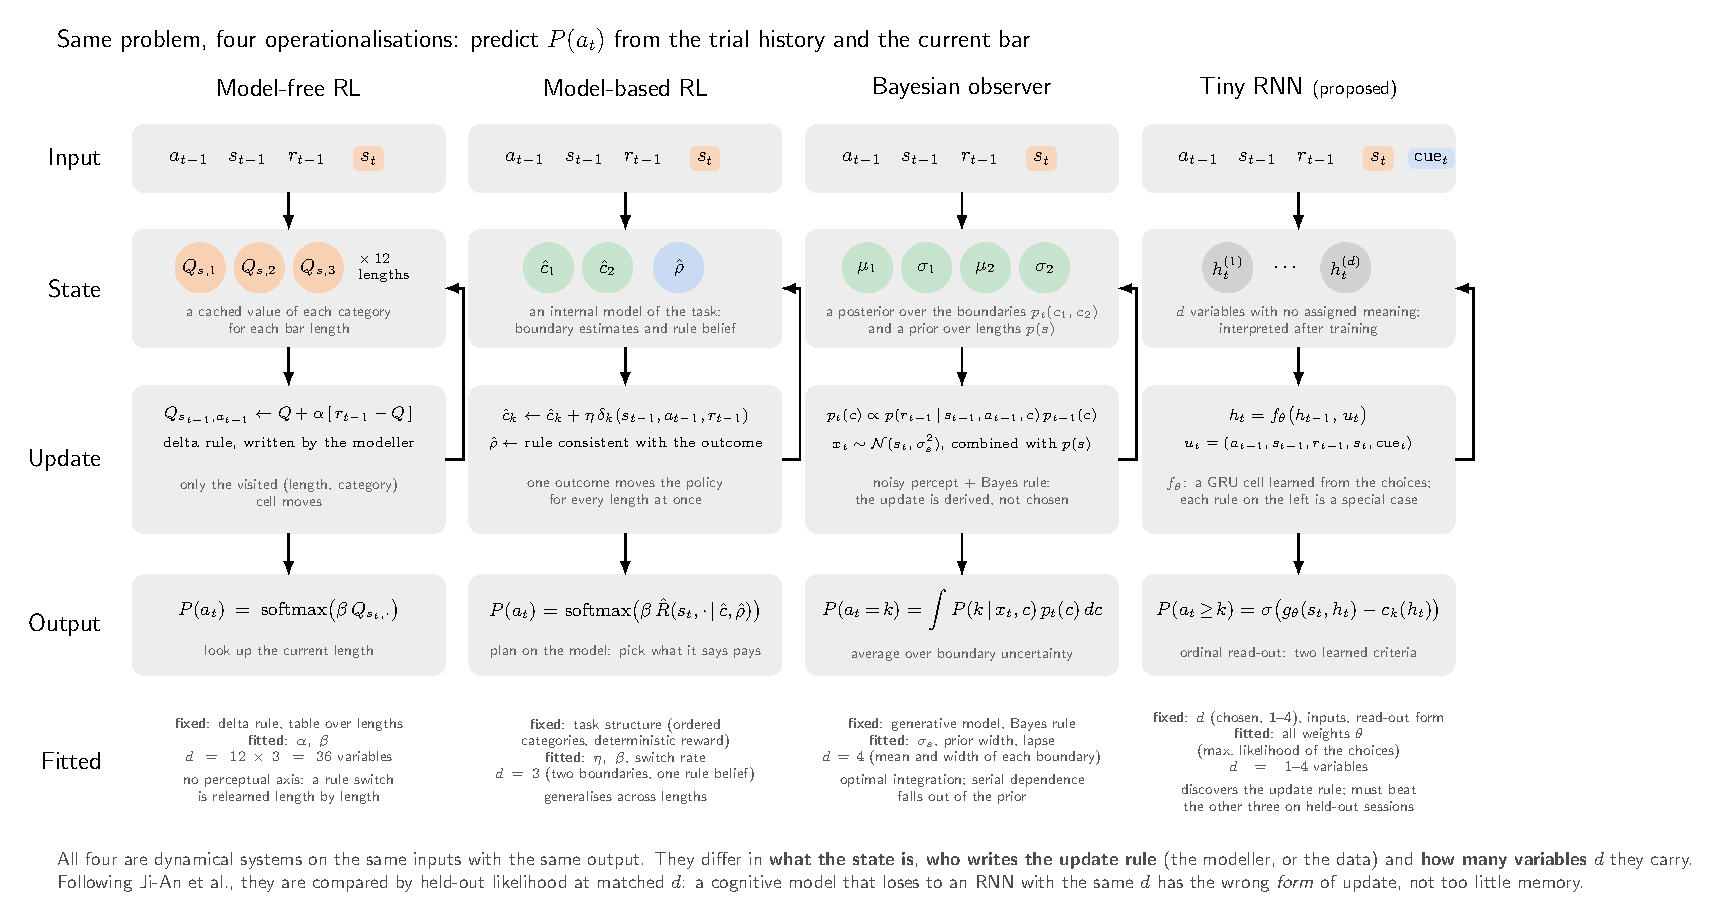
\includegraphics[width=\textwidth]{panel_f.pdf}
  \caption{Four operationalisations of the same problem. All four are dynamical systems
  on the same inputs with the same output. They differ in what the state is, in who
  writes the update rule (the modeller, a derivation, or the data) and in how many
  variables $d$ they carry. Following Ji-An et al., they are compared by held-out
  likelihood at matched $d$: a cognitive model that loses to a network with the same
  $d$ has the wrong form of update, not too little memory.}
  \label{fig:four}
\end{figure}

\subsection{Formal definitions}

\paragraph{M0, psychometric function without memory ($d=0$).} Equations
\eqref{eq:ro-x}--\eqref{eq:ro-cat} with $\vect{w}_g = \vect{w}_1 = \vect{w}_2 = 0$:
four parameters $c_1^0, \delta^0, \beta, \lambda$. Every gain is measured against this
floor.

\paragraph{M1, one trial back ($d=0$).} M0 plus linear terms in the previous trial,
\begin{equation}
  \hat{x}_t = s_t + \gamma_s\, s_{t-1} + \vect{\gamma}_a\T \mathrm{onehot}(a_{t-1})
              + \gamma_r\, r_{t-1} + \gamma_{ar}\, r_{t-1}\,\mathrm{sign}(a_{t-1} - \bar a),
\end{equation}
which separates ``there is an effect of the previous trial'' from ``the effect
accumulates''.

\paragraph{M2, criterion shift (the main cognitive model, $d=2$).} The two criteria are
the state. After each trial they move towards the previous stimulus if the choice was
wrong and decay towards a resting value:
\begin{equation}
  c_{k,t} = c_{k,t-1} + \eta\,(1 - r_{t-1})\,\operatorname{sign}(s_{t-1} - c_{k,t-1})\,
            \mathbb{1}\!\left[\,|s_{t-1} - c_{k,t-1}| < w\,\right]
            - \rho\,(c_{k,t-1} - c_k^{0}),
  \label{eq:m2}
\end{equation}
with learning rate $\eta$, window $w$ and decay $\rho$, and the read-out of
Eq.~\eqref{eq:ro-p}. This is the analogue of the ``value'' update of Ji-An et al.,
written for perceptual criteria.

\paragraph{M3, model-free reinforcement learning ($d = 36$).} A table
$Q_t(s, a)$ over the 12 lengths and 3 categories, updated by the delta rule
$Q_t(s_{t-1}, a_{t-1}) = Q_{t-1}(s_{t-1}, a_{t-1}) + \alpha\,[r_{t-1} - Q_{t-1}(s_{t-1}, a_{t-1})]$
and read out by $P(a_t) = \operatorname{softmax}(\beta\, Q_t(s_t, \cdot))$. It has no
perceptual axis: a rule switch must be relearned length by length.

\paragraph{M4, Bayesian observer ($d = 4$).} A Gaussian posterior over each criterion,
$c_k \sim \mathcal{N}(\mu_k, \sigma_k^2)$, updated by Bayes' rule with the likelihood
of the observed outcome, $p_t(c) \propto p(r_{t-1} \mid s_{t-1}, a_{t-1}, c)\,p_{t-1}(c)$;
a noisy percept $x_t \sim \mathcal{N}(s_t, \sigma_s^2)$ combined with a prior $p(s)$
over lengths; and a decision that averages over the posterior,
$P(a_t = k) = \int P(k \mid x_t, c)\,p_t(c)\,dc$. The update is derived, not chosen;
serial dependence falls out of the prior.

\begin{table}[H]
  \centering\small
  \caption{Models compared. All share the inputs, the output and the loss.}
  \label{tab:models}
  \begin{tabular}{lp{5.2cm}cp{5cm}}
    \toprule
    Model & State & $d$ & Establishes \\
    \midrule
    M0 psychometric & none & 0 & floor without memory \\
    M1 one trial back & none; previous-trial terms & 0 & effect versus accumulation \\
    M2 criterion shift & $c_1, c_2$ with Eq.~\eqref{eq:m2} & 2 & the hand-written analogue of value \\
    M3 model-free RL & $Q(s,a)$ table & 36 & reference without a perceptual axis \\
    M4 Bayesian & posterior mean and width per criterion & 4 & derived update \\
    RNN-plain & plain RNN & 1--4 & whether gates are needed \\
    RNN-GRU & this specification & 1--4 & \\
    Shuffled & RNN-GRU with permuted labels & & floor of the NLL \\
    \bottomrule
  \end{tabular}
\end{table}

\subsection{Decision rule}

The network ``discovers something'' only if it beats M1 and M2 with equal or smaller
$d$, in test NLL, with the bootstrap interval excluding zero. If it does not beat M1,
the past acts for one trial and does not accumulate. If it beats M1 but not M2, the
criterion model already captures the dynamics and is the model to report.

%======================================================================
\section{Interpretation}
\label{sec:interp}
%======================================================================

Once trained, the network is read on the stimulus axis, not on the state axis.

\begin{enumerate}[leftmargin=*]
\item \textbf{Criterion trajectories.} For every trial, $c_1(\vect{h}_t)$ and
      $c_2(\vect{h}_t)$ in degrees of visual angle, plotted against trial number with the
      block switches marked. This is the empirical version of the lower plots of
      Figure~\ref{fig:rule}.
\item \textbf{Phase portrait in criterion units.} With $d = 1$: $c_k(\vect{h}_t)$
      against $c_k(\vect{h}_{t-1})$, one curve per input condition (correct/error
      $\times$ previous category). Where a curve crosses the diagonal there is a fixed
      point; its slope says how much is retained. This is the plot of Ji-An et al.\
      transferred to length units.
\item \textbf{Gates.} Distribution of $z_t$ and $r_t$ by condition. A mean $z_t$ near 1
      confirms short memory; $r_t$ near 0 on the trials after a block switch confirms a
      reset.
\item \textbf{Input ablations.} Remove $s_{t-1}$, $a_{t-1}$, $r_{t-1}$ or $\cue_t$ one at
      a time and measure the loss in NLL. This quantifies the three sources of the past:
      perceptual serial dependence, feedback-driven criterion shift, and rule.
\item \textbf{Perception versus decision.} Relative magnitude of $\vect{w}_g$ against
      $\vect{w}_1, \vect{w}_2$: whether the past acts on perception or on the criterion.
\item \textbf{Closed form.} If $d = 1$, fit a simple expression (piecewise linear or a
      low-order polynomial) to the learned update curve. If it differs from
      Eq.~\eqref{eq:m2}, it is a new cognitive rule.
\item \textbf{Chronometric check.} In the joint model, observed decision time against
      $|\hat{x}_t - c_k(\vect{h}_t)|$ for the nearest criterion, binned. The curve must
      fall with distance; its slope is $\kappa$ in Eq.~\eqref{eq:dt-mu}.
\end{enumerate}

%======================================================================
\section{Predictions}
%======================================================================

\begin{table}[H]
  \centering\small
  \caption{Concrete predictions and their basis. Any of these that fails is a result,
  not a problem with the model.}
  \begin{tabular}{p{9.5cm}p{5.5cm}}
    \toprule
    Prediction & Basis \\
    \midrule
    M1 beats M0 by a small margin: the post-error effect exists & accuracy 0.69 versus 0.79 \\
    RNN $d=1$ matches or beats M1 by a small margin; $d=2$ does not improve on $d=1$ in three-category sessions & weak sequential effects \\
    Mean $z_t > 0.5$: memory of one or two trials & fixed rule, deterministic reward \\
    Fitted $c_1$ near 4.6, below the nominal 5.05; $c_2$ near 6.4 & Table~\ref{tab:psycho} \\
    On the five trials after each block switch the cue-driven version beats the latent one; the latent version closes the gap within about ten trials & the cue is visible; the split moves a boundary by 0.8 deg VA, which errors reveal quickly \\
    The between-session NLL exceeds the within-session NLL by less than the gap between M0 and the best RNN & accuracy stable at 0.73--0.81 across days \\
    Ablating $s_{t-1}$ costs more NLL than ablating $a_{t-1}$ & perceptual serial dependence is the typical history effect in categorization \\
    In the joint model $\kappa > 0$: decision times peak near the fitted criteria & chronometric effect, notebook Section 1.6 \\
    The joint model reaches the same choice NLL as the choice-only model with fewer sessions & the decision time is a continuous second observation per trial \\
    \bottomrule
  \end{tabular}
\end{table}

%======================================================================
\section{Data requirements and changes to the task}
\label{sec:data-req}
%======================================================================

The design assumes that \texttt{alternate} is the base session mode from now on.
Table~\ref{tab:datareq} lists what that corpus has to look like for the split of
Section~\ref{sec:split} to work, and what has to change in the task code.

\begin{table}[H]
  \centering\small
  \caption{What the analysis needs from future sessions.}
  \label{tab:datareq}
  \begin{tabular}{p{3.8cm}p{4.2cm}p{7cm}}
    \toprule
    Need & Current state & What is required \\
    \midrule
    Enough \texttt{alternate} sessions & 1 session, 6 switches & 12 to 15 sessions, 50 to 70 switches in total (Section~\ref{sec:type}); ten is the floor for the latent-rule version \\
    Variable segment length & fixed at one block (48 trials) per segment & draw \texttt{alternateBlocks2cat} and \texttt{alternateBlocks3cat} independently from $\{1, 2, 3\}$ with weights about $0.6/0.3/0.1$ for every session, so the rule cannot be predicted by counting trials and switches stay frequent \\
    Both switch directions & 2$\to$3 and 3$\to$2 both present & keep alternating the starting rule across sessions so the two directions are balanced \\
    A stable two-category split & marked ``placeholder'' in \texttt{ConfigBarLengths.m} & fix it: the model assumes $c_1^{\mathrm{2cat}}$ is the same in every session \\
    Motor bias separated from decision bias & the target layout is not exported & export the category at each of the four positions; \texttt{PrevTrialDirection} then becomes an input channel \\
    Uniform schema & old sessions lack \texttt{NumCategories} & the notebook's normaliser already handles it; document it in the export \\
    \bottomrule
  \end{tabular}
\end{table}

%======================================================================
\section{Relation to the within-trial networks}
\label{sec:within}
%======================================================================

The companion document specifies two networks that operate inside the trial at a
10 ms step: a continuous-time rate network that reads the category out over the trial,
and a GRU that produces the cursor trajectory (Figure~\ref{fig:unrolled}). Three links
tie them to the network specified here.

\begin{itemize}[leftmargin=*]
\item The curve $s_t \mapsto P(a_t)$ of this network, evaluated at a typical
      $\vect{h}_t$, must agree with the asymptotic output $z(T)$ of the task network.
      If they disagree, one of the two is absorbing something that is not its own.
\item The state $\vect{h}_t$ can serve as the initial condition of the task network on
      trial $t$, giving it history context it need not learn. This is optional and is
      evaluated as an ablation.
\item This network is fitted first. It is the cheapest, it fixes the minimal $d$ of
      history, and it says whether there is a history the other networks must respect.
\end{itemize}

\begin{figure}[htbp]
  \centering
  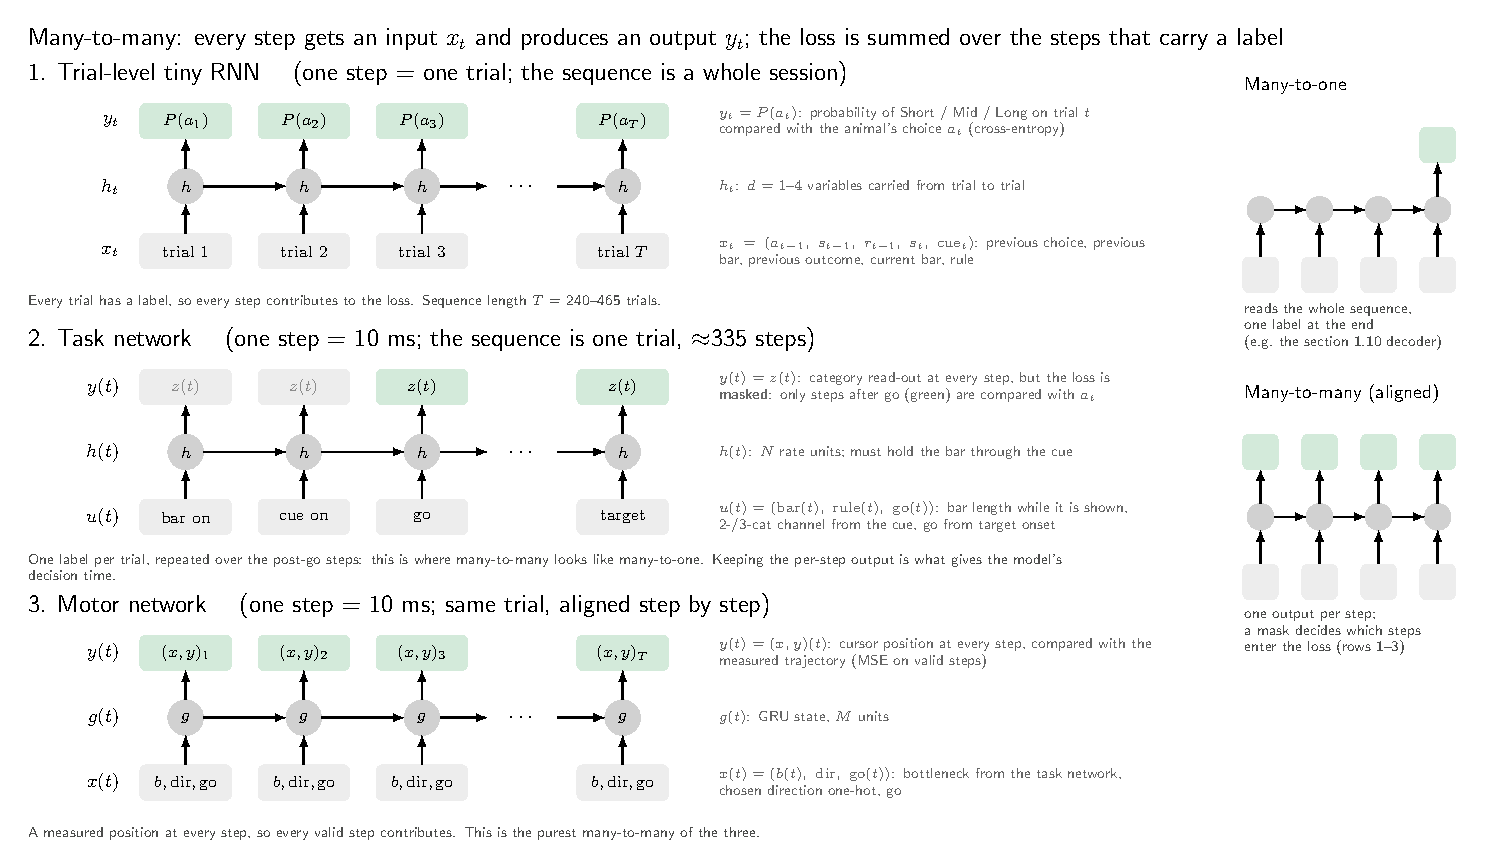
\includegraphics[width=\textwidth]{panel_g.pdf}
  \caption{The three networks unrolled in time, with what $x_t$ and $y_t$ are in each.
  Row 1 is this document's network (one step per trial, every step labelled). Rows 2 and
  3 are the within-trial task and motor networks (one step per 10 ms); the task network's
  outputs before the go signal are masked, which is where many-to-many looks like
  many-to-one, and the motor network has a measured position at every step. Right: the
  two topologies contrasted.}
  \label{fig:unrolled}
\end{figure}

\clearpage
%======================================================================
\appendix
\section{Model skeleton in PyTorch}
%======================================================================

The choice loss is \texttt{-(mask * log probs[a\_obs]).sum() / mask.sum()}; the
decision-time loss is the Gaussian negative log-likelihood of \texttt{log\_dt} given
\texttt{mu} and \texttt{log\_sd.exp()}, with the same mask, weighted by
$\lambda_{\mathrm{RT}}$. For the feedback-inferred version the two $\cue_t$ channels of
\texttt{x} are set to zero; for the choice-only model the second output is ignored.

\begin{lstlisting}
import torch, torch.nn as nn, torch.nn.functional as F

class TinyRNN(nn.Module):
    def __init__(self, k=9, d=1, link="logistic"):
        super().__init__()
        self.cell = nn.GRUCell(k, d)
        self.h0   = nn.Parameter(torch.zeros(d))
        self.w_g  = nn.Linear(d, 1)          # x_hat = s_t + w_g.h + b_g
        self.w_c  = nn.Linear(d, 2)          # c_1, delta  (c_2 = c_1 + softplus(delta))
        self.log_beta  = nn.Parameter(torch.zeros(1))
        self.lapse_raw = nn.Parameter(torch.tensor(-3.0))
        self.link = link
        # decision-time head (Sec. Decision time): mu = mu0 + kappa * D + w_dt.h
        self.w_dt   = nn.Linear(d, 1)
        self.kappa  = nn.Parameter(torch.zeros(1))
        self.log_sd = nn.Parameter(torch.zeros(1))

    def cdf(self, u):
        if self.link == "logistic":
            return torch.sigmoid(u)
        return 0.5 * (1 + torch.erf(u / 2 ** 0.5))   # cumulative Gaussian

    def forward(self, x, s):                  # x: (T, B, k), s: (T, B)
        T, B, _ = x.shape
        h = self.h0.expand(B, -1)
        out, mu = [], []
        for t in range(T):
            h = self.cell(x[t], h)
            xhat = s[t] + self.w_g(h).squeeze(-1)
            c = self.w_c(h)
            c1 = c[:, 0]
            c2 = c1 + F.softplus(c[:, 1])
            beta = self.log_beta.exp()
            lam = 0.1 * torch.sigmoid(self.lapse_raw)
            p1 = (1 - lam) * self.cdf(beta * (xhat - c1)) + lam / 2   # P(a >= 1)
            p2 = (1 - lam) * self.cdf(beta * (xhat - c2)) + lam / 2   # P(a >= 2)
            probs = torch.stack([1 - p1, p1 - p2, p2], dim=-1).clamp_min(1e-6)
            out.append(probs)
            D = -torch.minimum((xhat - c1).abs(), (xhat - c2).abs())   # Eq. (dt-D)
            mu.append(self.w_dt(h).squeeze(-1) + self.kappa * D)
        return torch.stack(out), torch.stack(mu)   # (T, B, 3), (T, B)
\end{lstlisting}

\end{document}
